% !TeX root = ../../thesis.tex
\chapter{Ambient Stability of Thermally Co-Evaporated \ch{CsPbI_2Br} Thin Films}\label{ch:stability}

Stabitlity of CsPbiXbR3-X has been primarily been einvesitgated for solution processed films

even though a drastically different crystallization mechanism 

some insights from solution prosesssec on the factors that affect are: 
 only a very limited studies refer to the stability of evaporated and the reporte stabilities are widelie diffrent 


Factors that affect ambient stability of the CsPbIxBr3-x system without the incorporation wihtout the incorporation of additives new elements in the lattice 

wihtout pursuing compositional changes


\section{Introduction}

\section{Benchmarking Ambient Stability}


\begin{figure}[htbp]
    \centering
    % First row
    \begin{subfigure}[t]{0.49\textwidth}
        \centering
        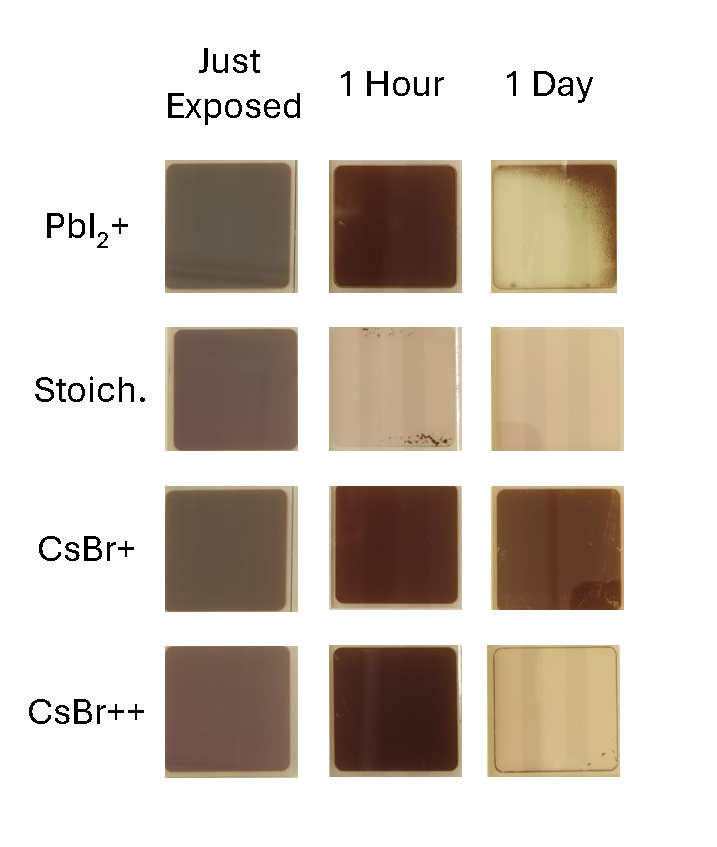
\includegraphics[width=\textwidth]{chapters/stability/imeges/Stability_Rotation_Stoichiometries.pdf} % Replace with your image file
        \caption*{(a)}
    \end{subfigure}
    \hfill
    \begin{subfigure}[t]{0.45\textwidth}
        \centering
        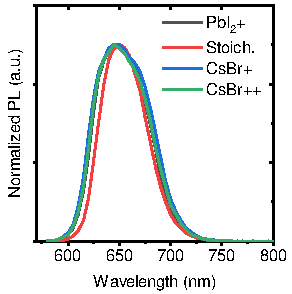
\includegraphics[width=\textwidth]{chapters/stability/imeges/PL_Normalized.pdf} % Replace with your image file
        \caption*{(b)}
    \end{subfigure}

    % Second row
    \begin{subfigure}[t]{0.99\textwidth}
        \centering
        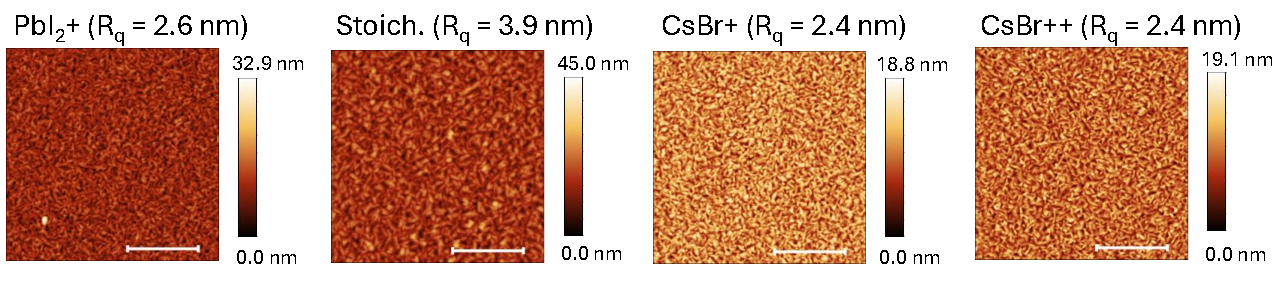
\includegraphics[width=\textwidth]{chapters/stability/imeges/Stability_Rotation_Stoich_AFM.pdf} % Replace with your image file
        \caption*{(c)}
    \end{subfigure}

    \caption{}
    \label{}
\end{figure}


\begin{figure}[htbp]
    \centering
    % Second row
    \begin{subfigure}[t]{0.7\textwidth}
        \centering
        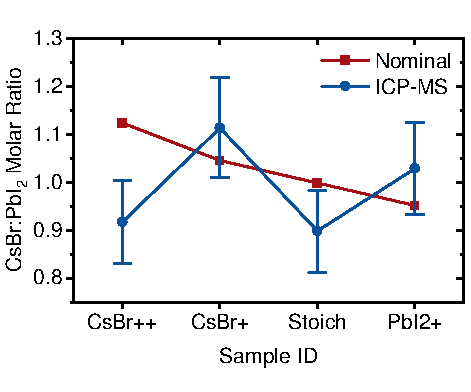
\includegraphics[width=\textwidth]{chapters/stability/imeges/Stability-ICP-MS.pdf} % Replace with your image file                
    \end{subfigure}

    \caption{}
    \label{}
\end{figure}


\begin{figure}[htbp]
    \centering
    % Second row
    \begin{subfigure}[t]{0.99\textwidth}
        \centering
        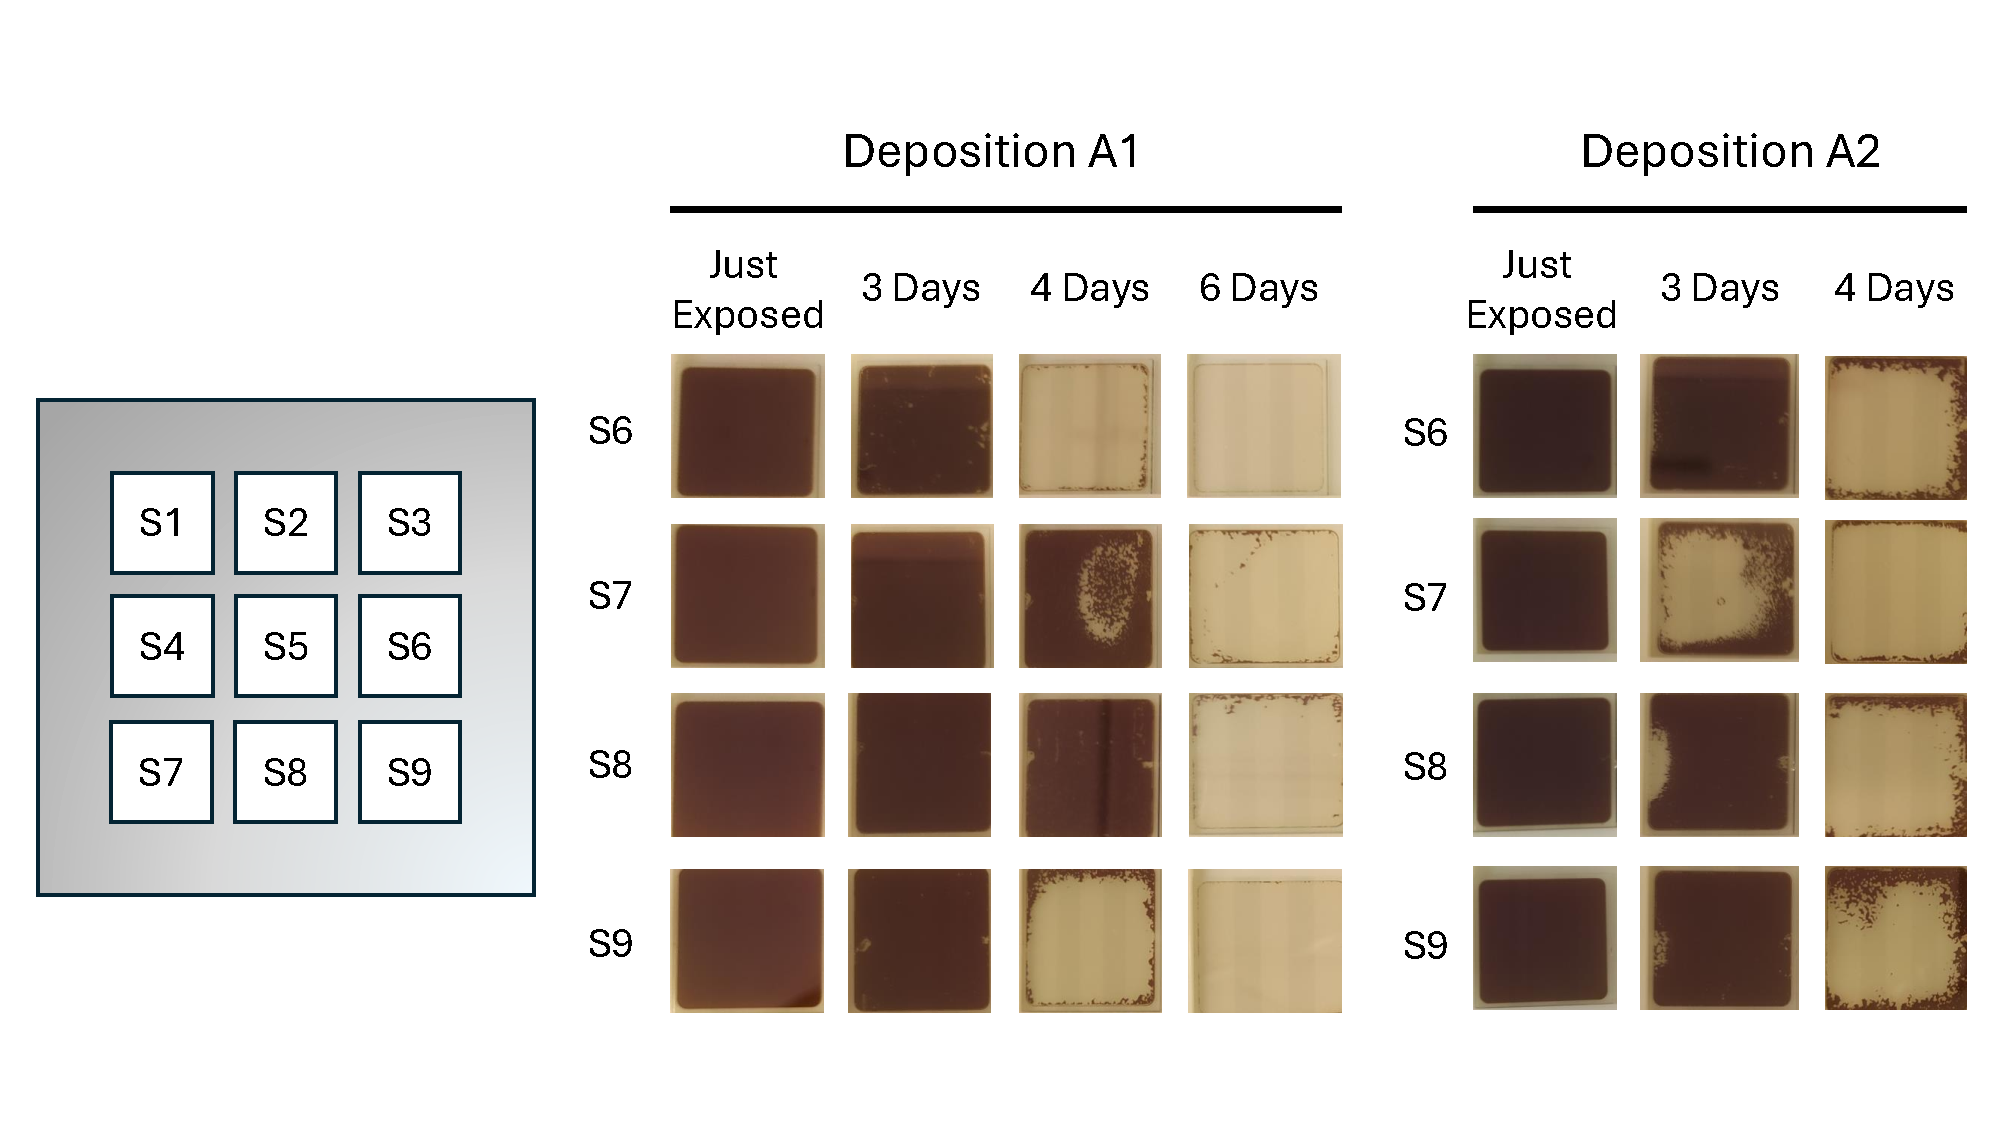
\includegraphics[width=\textwidth]{chapters/stability/imeges/Stability_Rotation_Repeatability.pdf} % Replace with your image file                
    \end{subfigure}
    \caption{}
    \label{}
\end{figure}



\section{Improving Ambient Stability through High-Throughout Experimentation}


\begin{figure}[htbp]
    \centering
    % First plot
    \begin{subfigure}[t]{0.49\textwidth} % Adjust width as needed
        \centering
        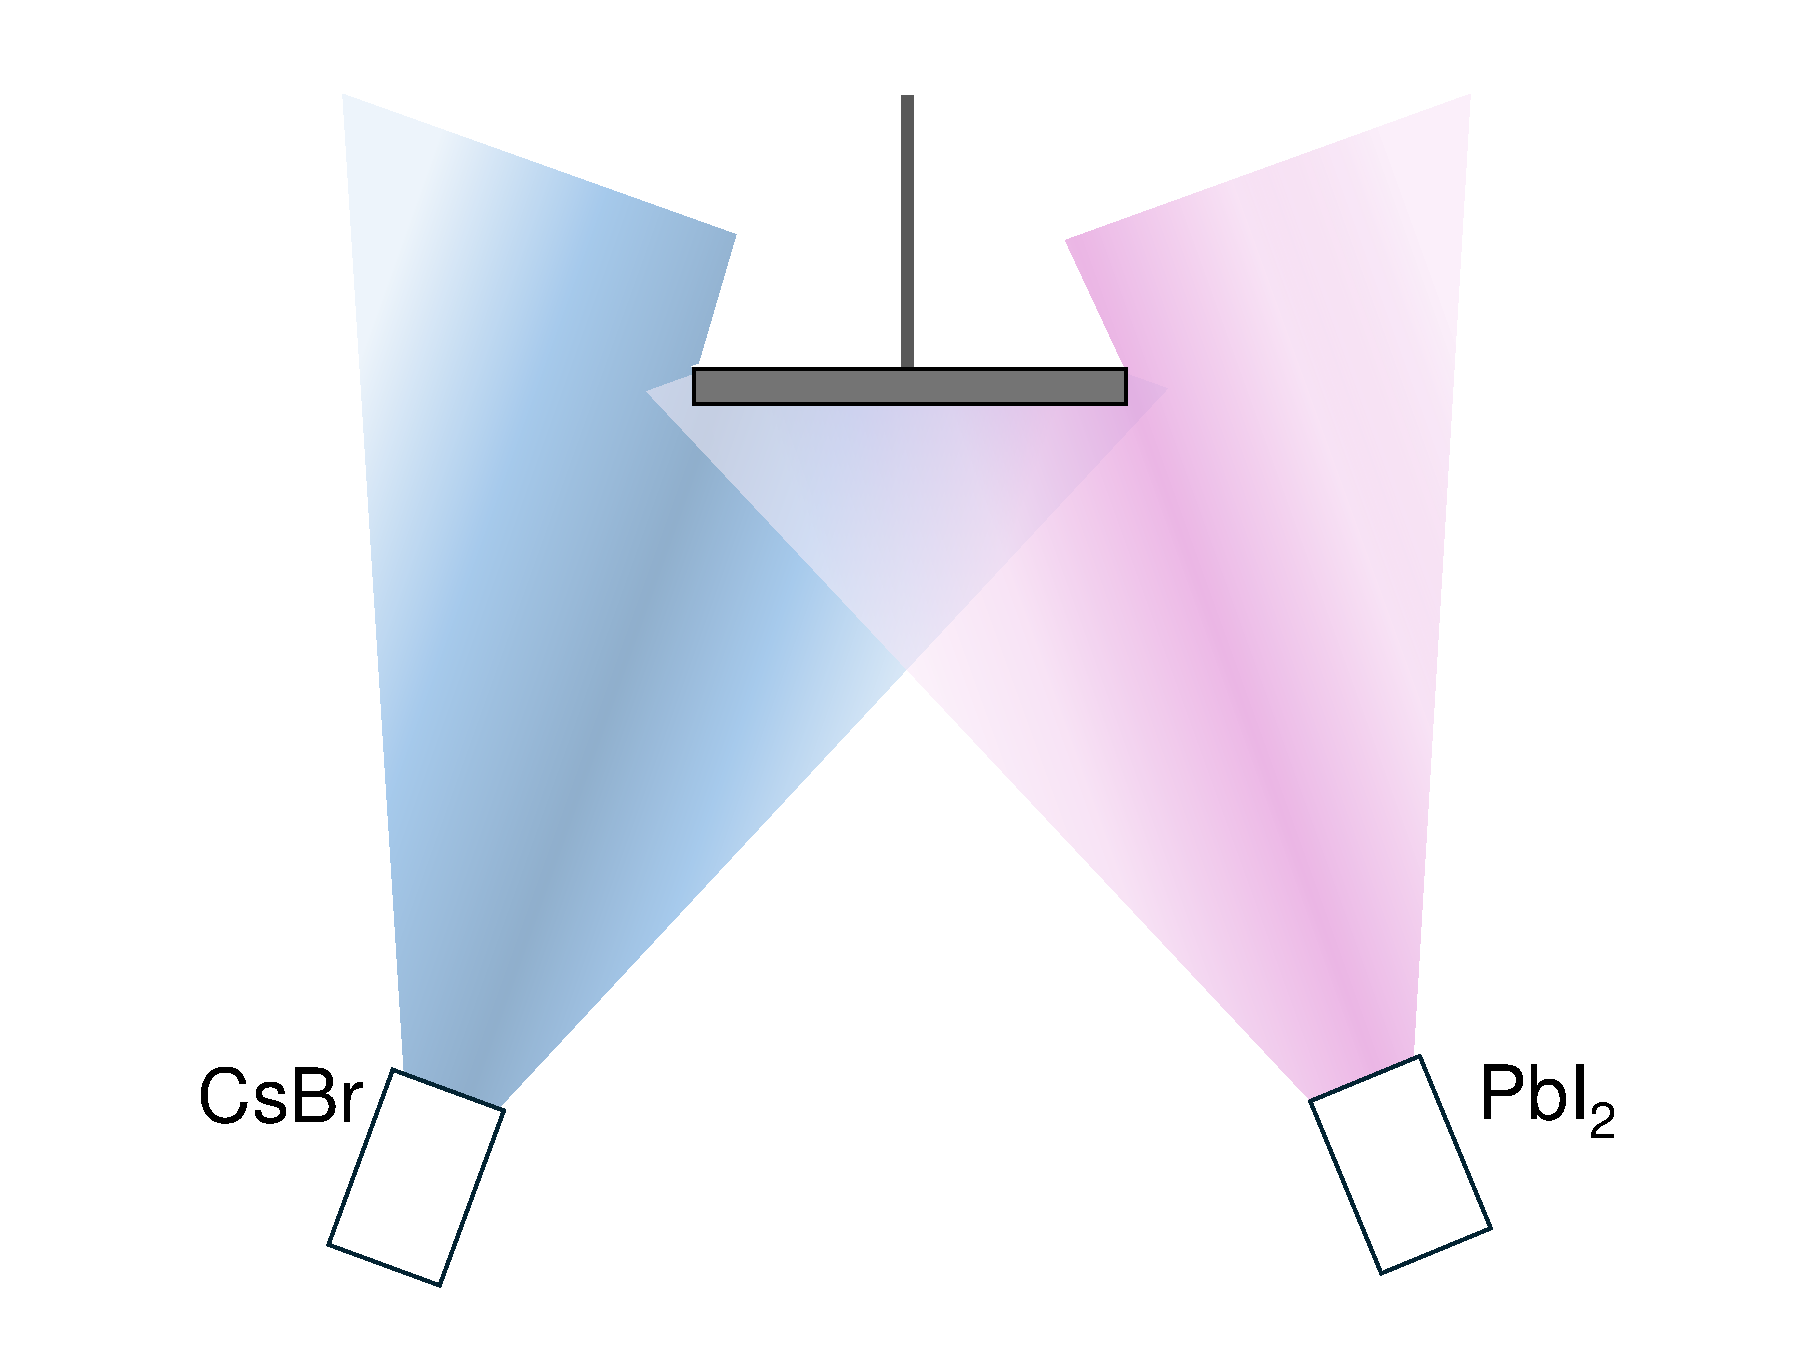
\includegraphics[width=\textwidth]{chapters/stability/imeges/Chamber - Side View.pdf} % Replace with your image
        \caption{}
        \label{}
    \end{subfigure}
    % Second plot
    \begin{subfigure}[t]{0.49\textwidth} % Adjust width as needed
        \centering
        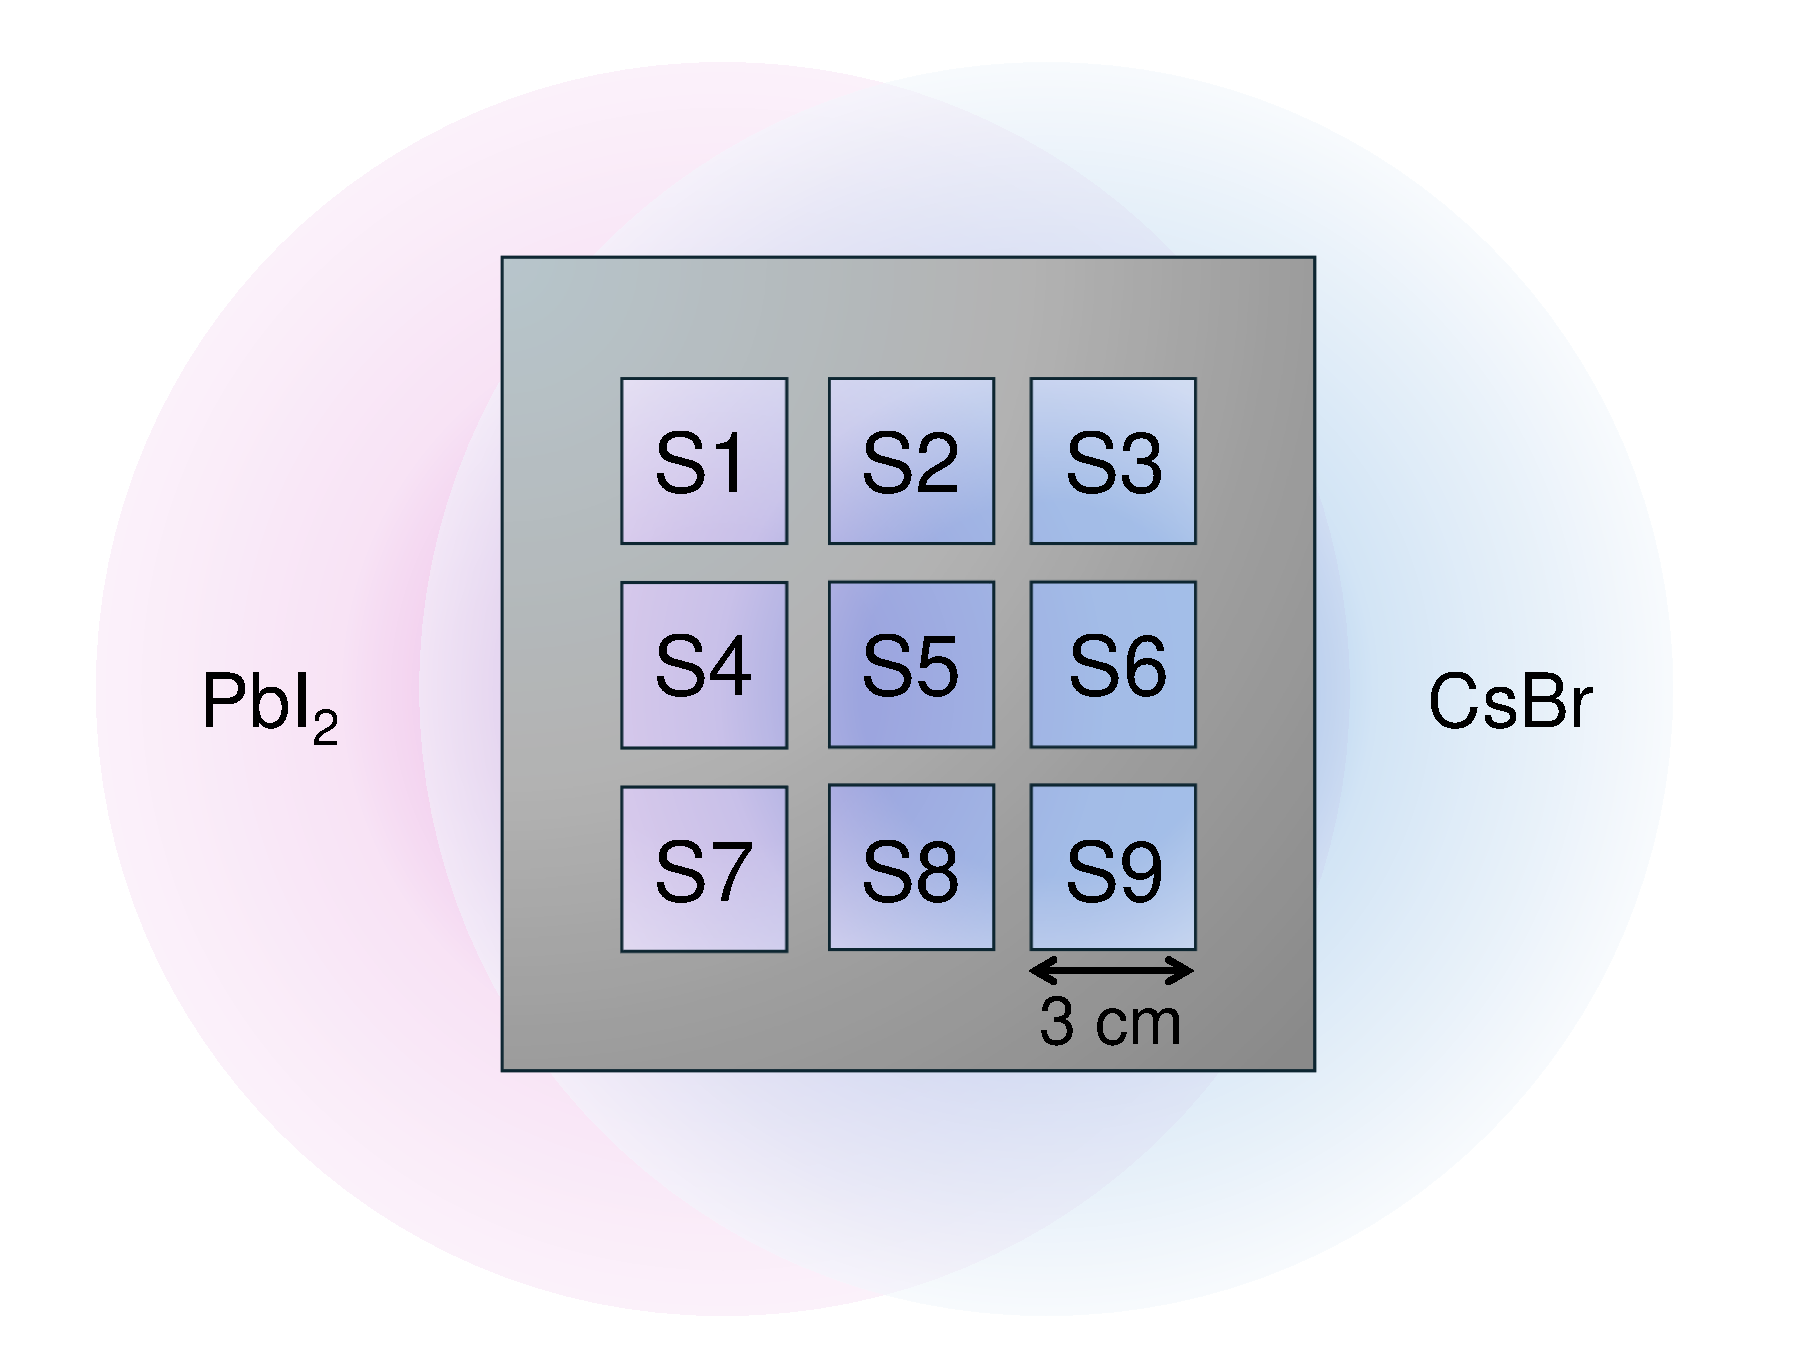
\includegraphics[width=\textwidth]{chapters/stability/imeges/Holder - Gradient - Schematic.pdf} % Replace with your image
        \caption{}        
        \label{}
    \end{subfigure}

    % Caption for the whole figure
    \caption{}   
    \label{}
\end{figure}


\begin{figure}[htbp]
    \centering
    % Second row
    \begin{subfigure}[t]{0.99\textwidth}
        \centering
        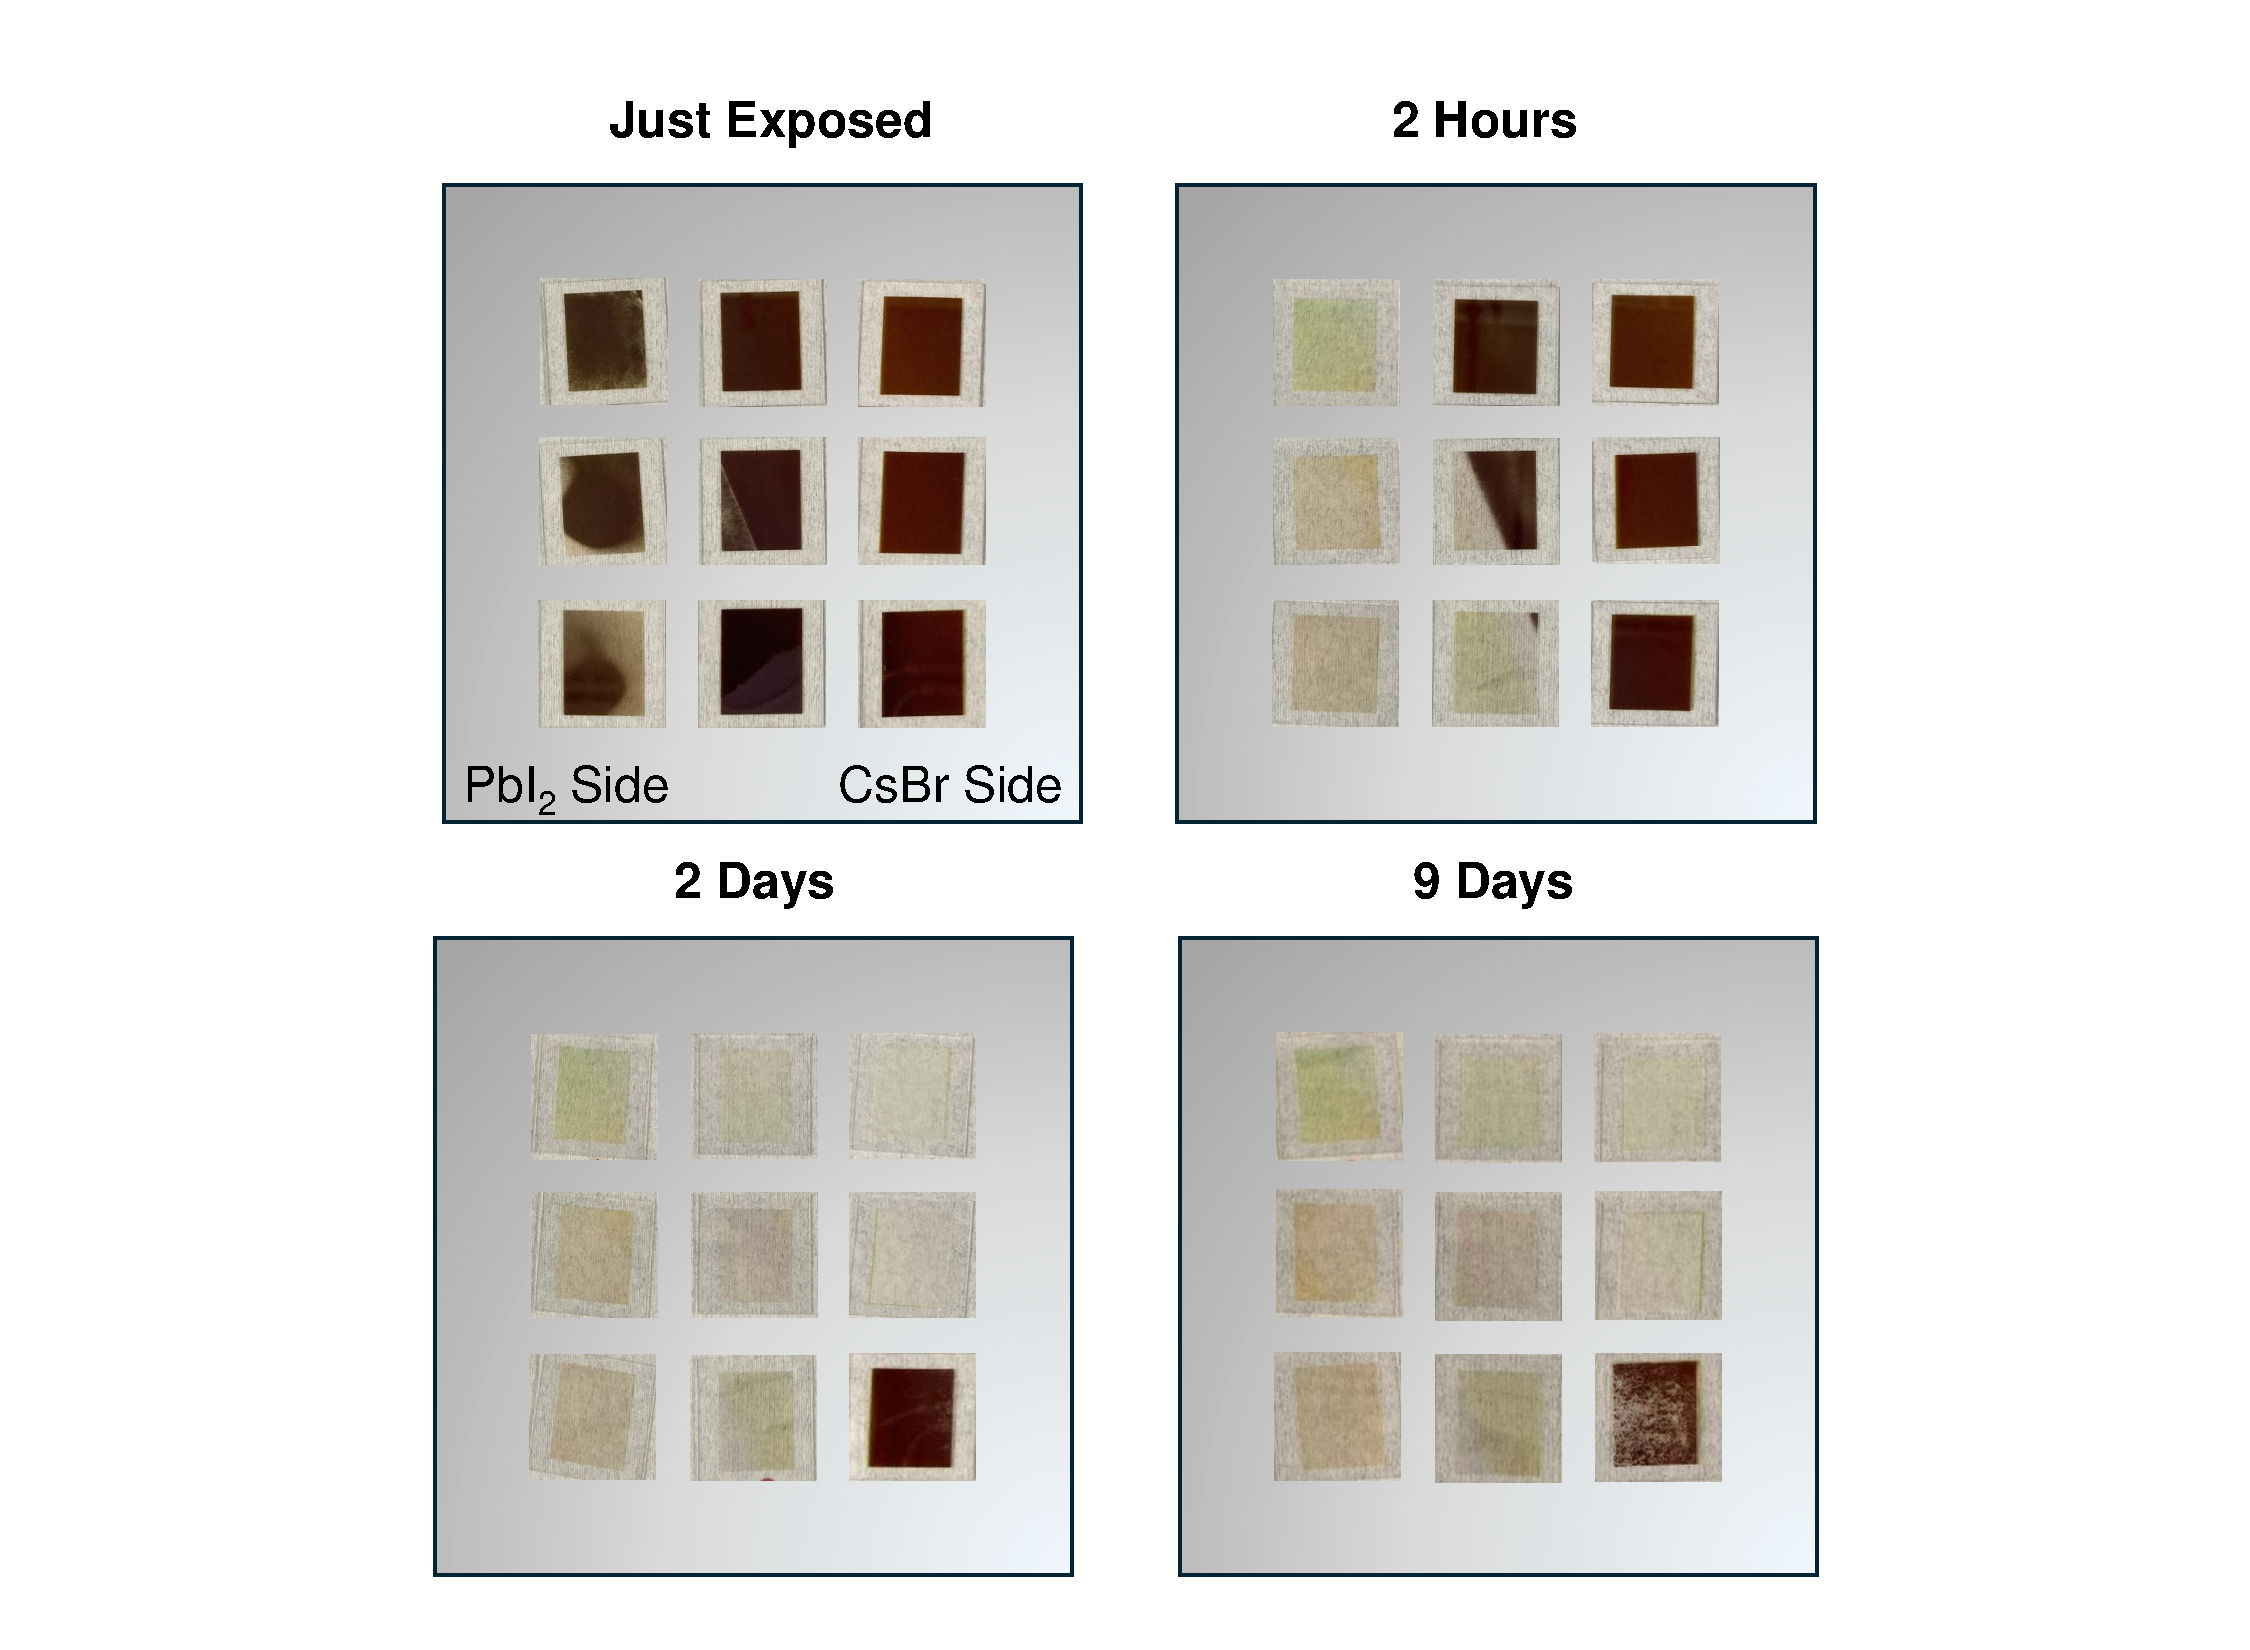
\includegraphics[width=\textwidth]{chapters/stability/imeges/Stability - No Rotation_275nm_on_glass.pdf} % Replace with your image file
                
    \end{subfigure}

    \caption{}
    \label{}
\end{figure}



\begin{figure}[htbp]
    \centering
    % Second row
    \begin{subfigure}[t]{0.99\textwidth}
        \centering
        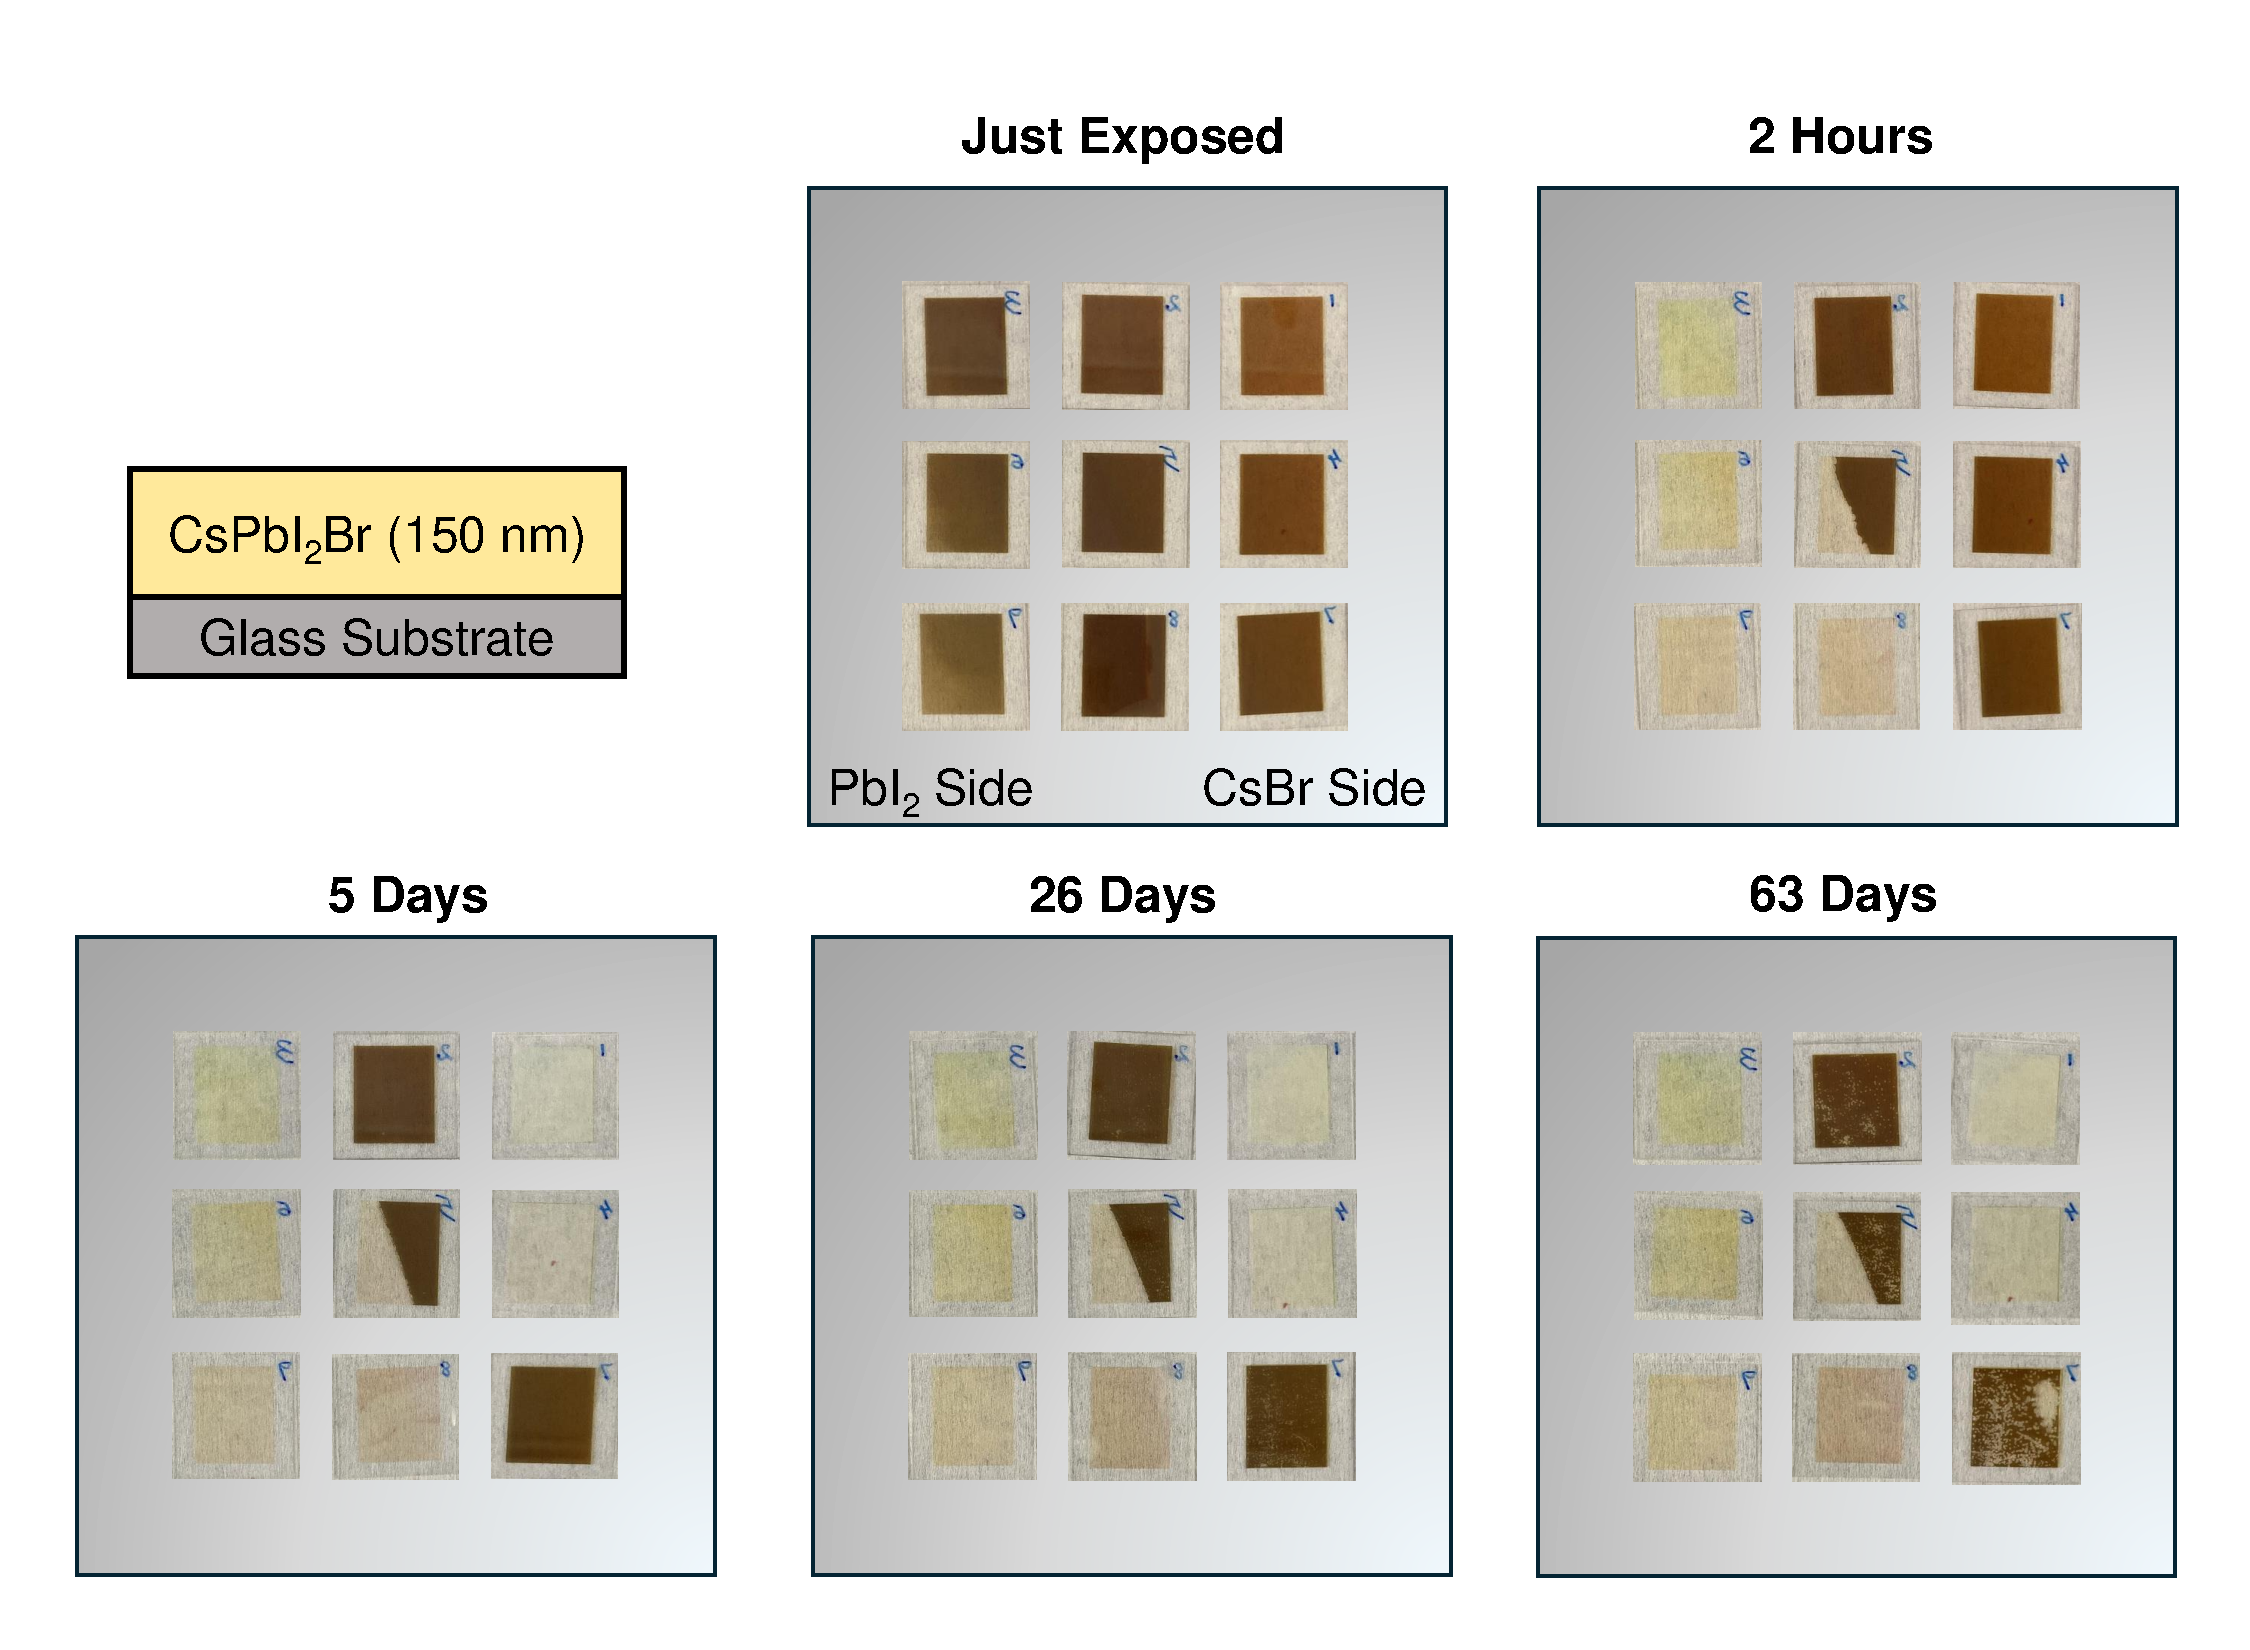
\includegraphics[width=\textwidth]{chapters/stability/imeges/Stability_No_Rotation_139nm_on_glass.pdf} % Replace with your image file                
    \end{subfigure}

    \caption{}
    \label{}
\end{figure}

\begin{figure}[htbp]
    \centering
    % Second row
    \begin{subfigure}[t]{0.99\textwidth}
        \centering
        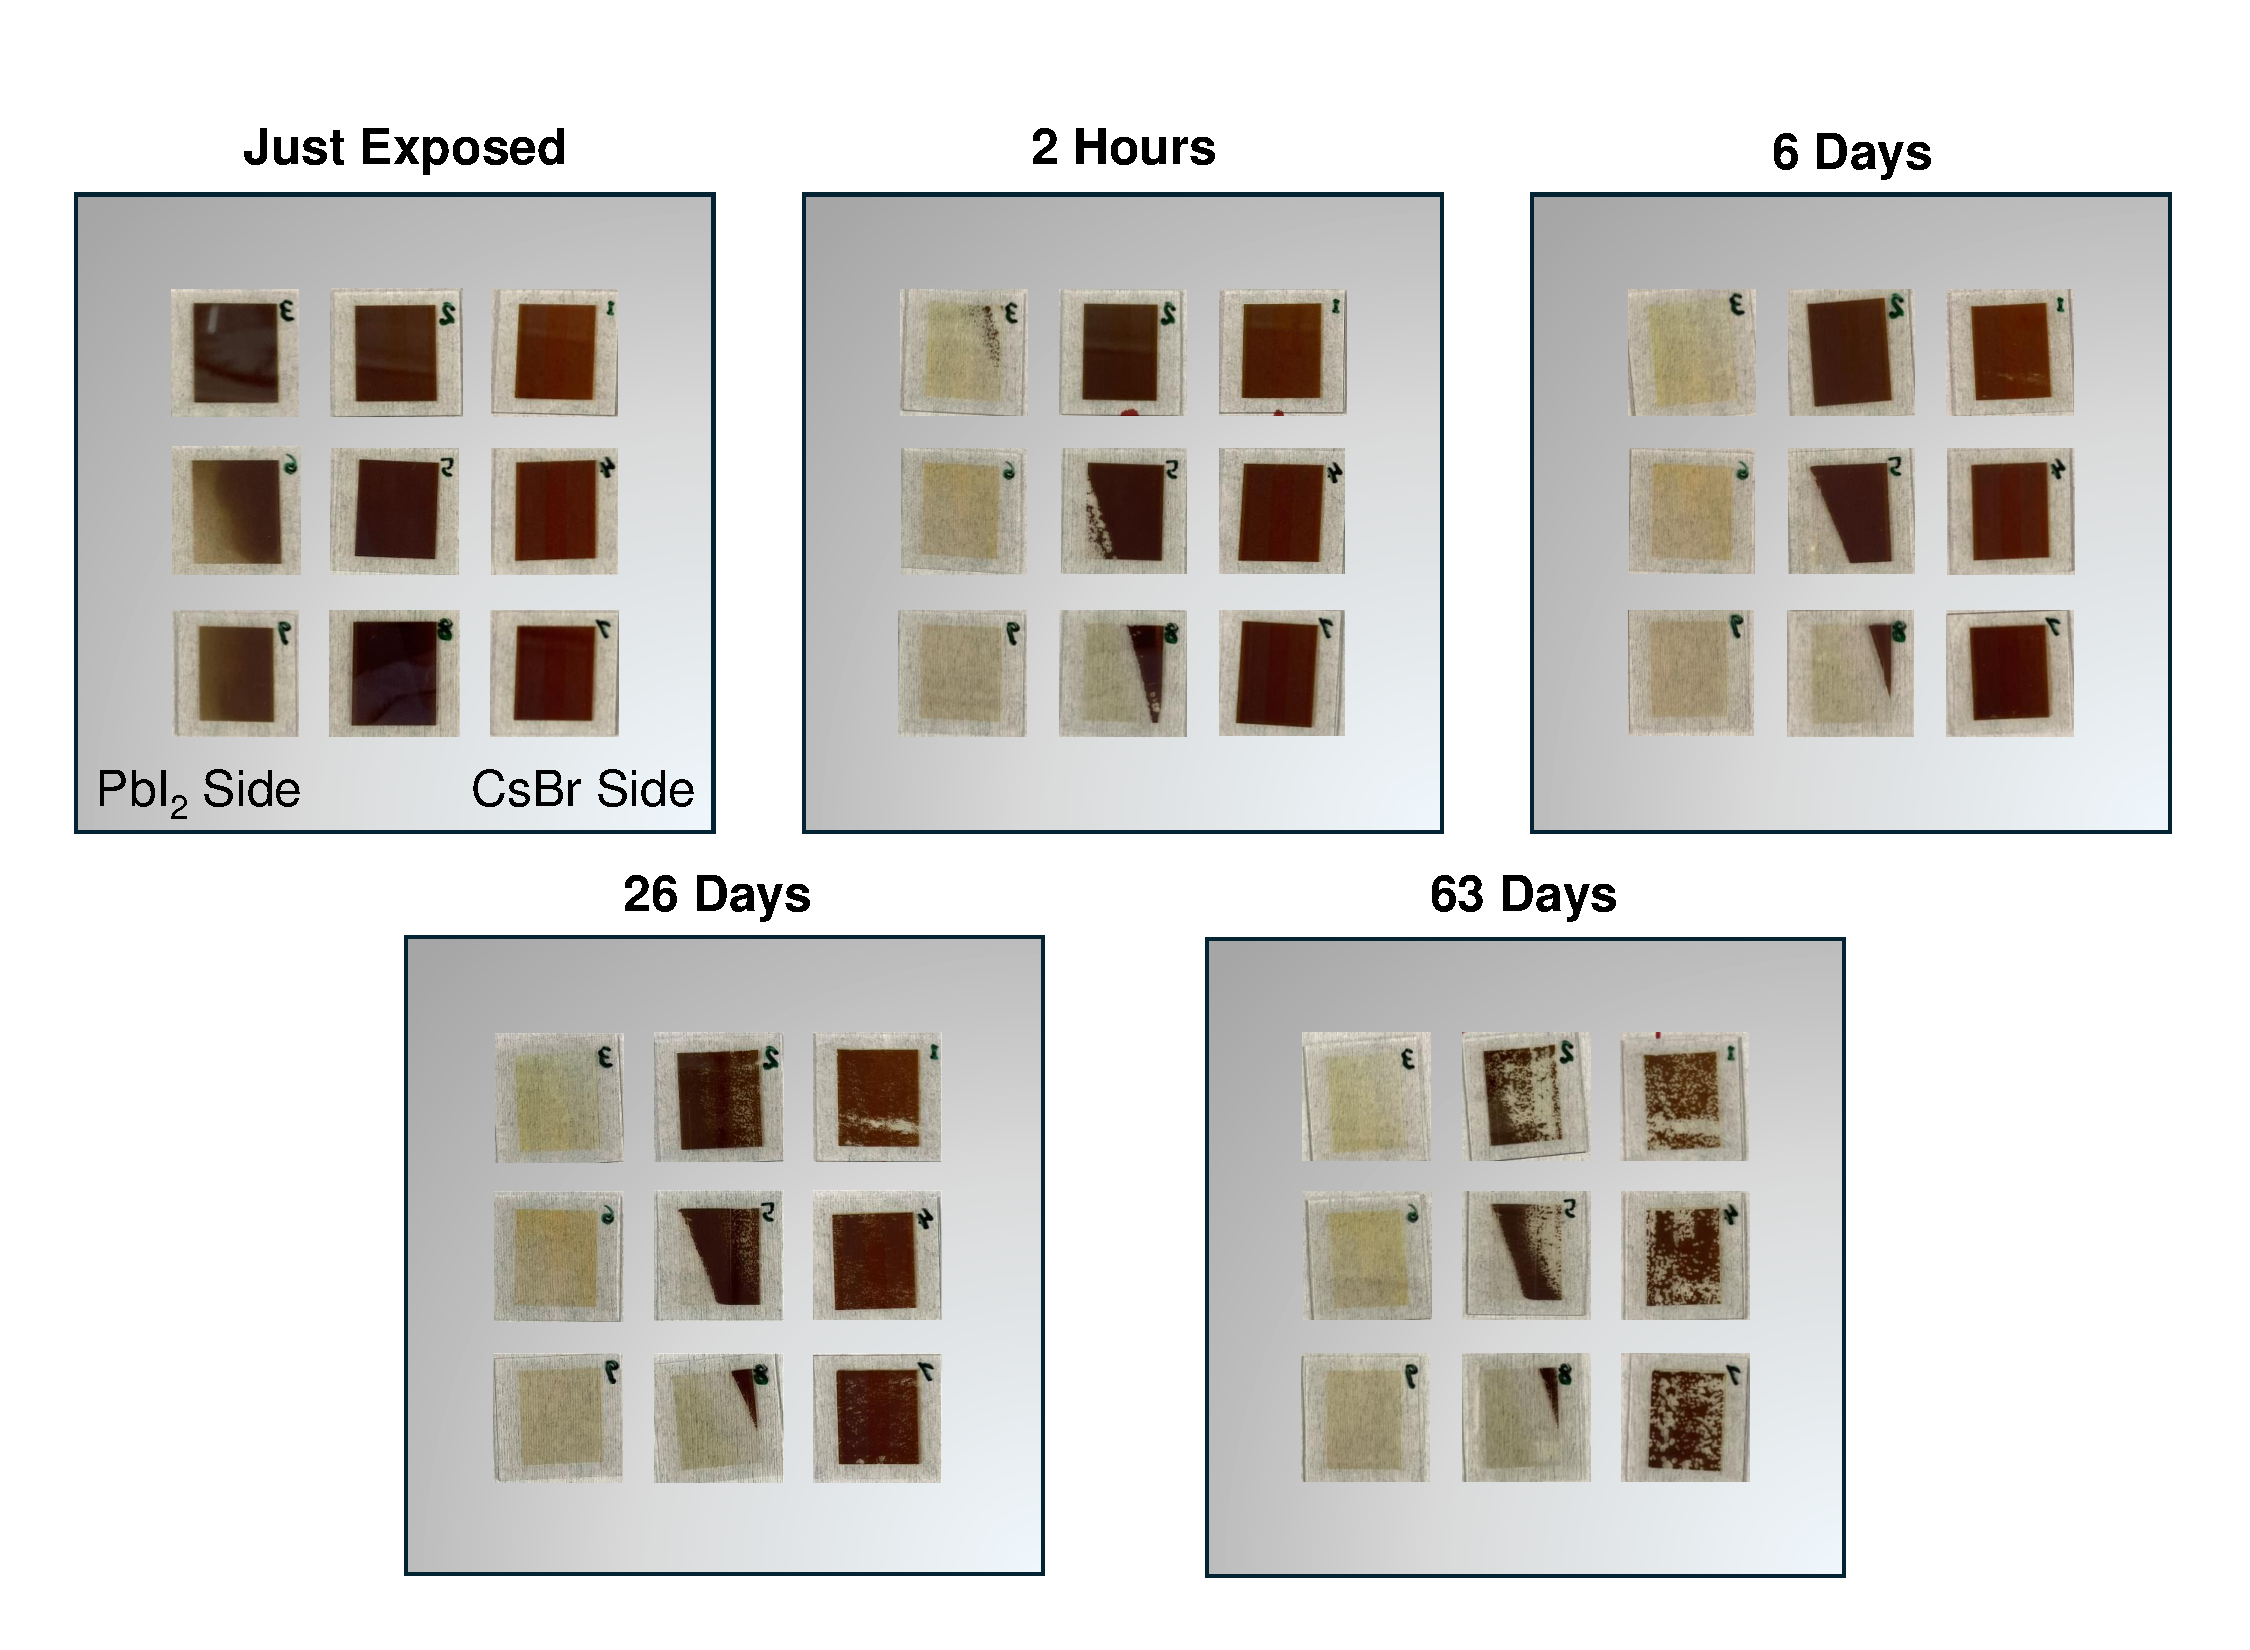
\includegraphics[width=\textwidth]{chapters/stability/imeges/Stability_No_Rotation_275_on_nio.pdf} % Replace with your image file                
    \end{subfigure}

    \caption{}
    \label{}
\end{figure}


\begin{figure}[htbp]
    \centering
    % First row
    \begin{subfigure}[t]{0.49\textwidth}
        \centering
        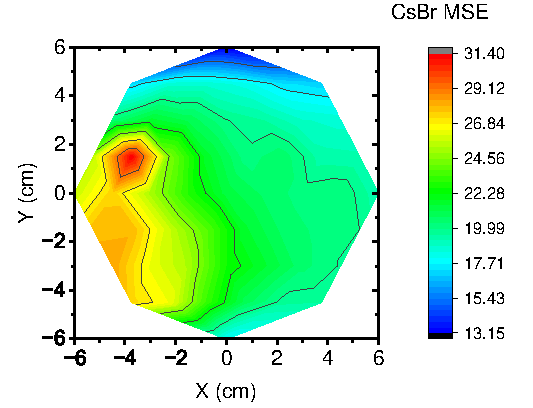
\includegraphics[width=\textwidth]{chapters/stability/imeges/CsBrMSE.pdf} % Replace with your image file
        \caption*{(a)}
    \end{subfigure}
    \hfill
    \begin{subfigure}[t]{0.49\textwidth}
        \centering
        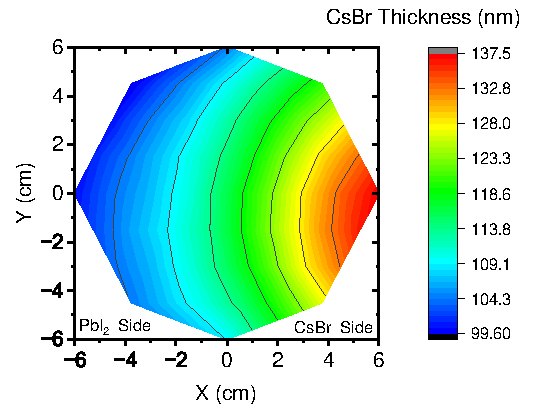
\includegraphics[width=\textwidth]{chapters/stability/imeges/CsBrThickness.pdf} % Replace with your image file
        \caption*{(b)}
    \end{subfigure}


    % Second row
    \begin{subfigure}[t]{0.49\textwidth}
        \centering
        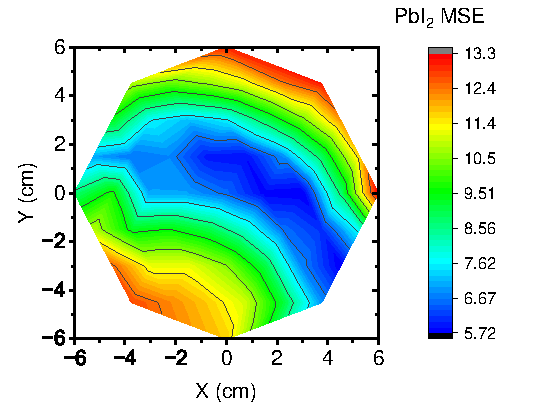
\includegraphics[width=\textwidth]{chapters/stability/imeges/PbI2MSE.pdf} % Replace with your image file
        \caption*{(c)}
    \end{subfigure}
    \hfill
    \begin{subfigure}[t]{0.49\textwidth}
        \centering
        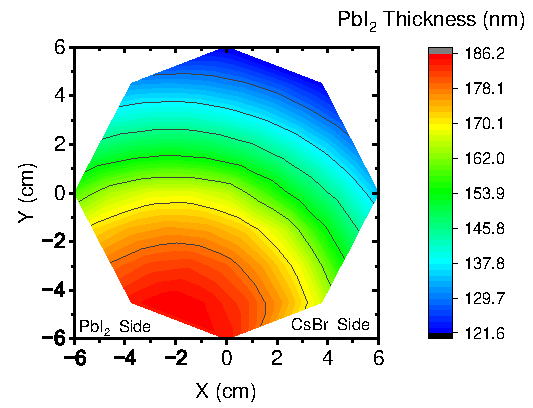
\includegraphics[width=\textwidth]{chapters/stability/imeges/PbI2Thickness.pdf} % Replace with your image file
        \caption*{(d)}
    \end{subfigure}
    \caption{}
    \label{}
\end{figure}


\begin{figure}[htbp]
    \centering
    % Second row
    \begin{subfigure}[t]{0.7\textwidth}
        \centering
        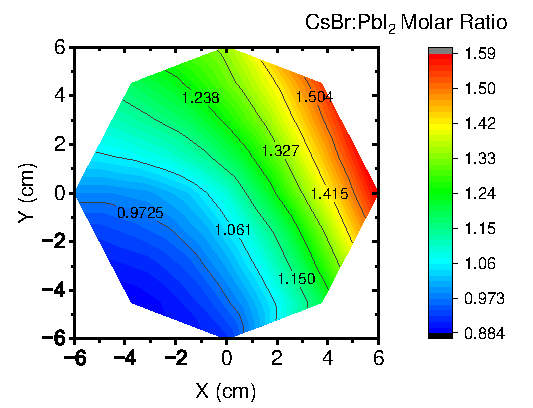
\includegraphics[width=\textwidth]{chapters/stability/imeges/Molar_Ratio.pdf} % Replace with your image file                
    \end{subfigure}

    \caption{}
    \label{}
\end{figure}


\section{Conclusions}

%%%%%%%%%%%%%%%%%%%%%%%%%%%%%%%%%%%%%%%%%%%%%%%%%%
% Keep the following \cleardoublepage at the end of this file, 
% otherwise \includeonly includes empty pages.
\cleardoublepage

